\documentclass[tikz,border=10pt]{standalone}
\usepackage{tikz}
\usepackage{amsmath}

\begin{document}
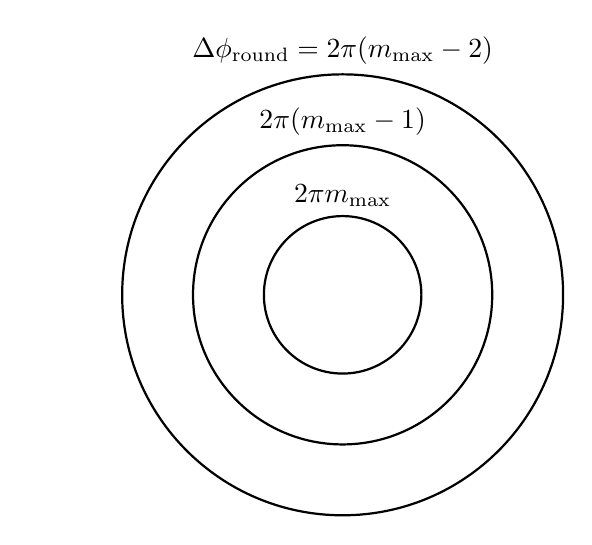
\begin{tikzpicture}

  % Left margin padding
  \path (-4, 0);

  % Three concentric circles (innermost to outermost)
  \draw[thick] (0,0) circle (1.0);
  \draw[thick] (0,0) circle (1.9);
  \draw[thick] (0,0) circle (2.8);

  % Labels above each circle, on the y-axis
  \node[above] at (0, 1.0) {$2\pi m_\text{max}$};
  \node[above] at (0, 1.9) {$2\pi (m_\text{max} - 1)$};
  \node[above] at (0, 2.8) {$\Delta \phi_\text{round} = 2\pi (m_\text{max} - 2)$};

\end{tikzpicture}
\end{document}
